% chktex-file 3
% chktex-file 8
% chktex-file 35
\section{First-principles shift-field derivation}\label{sec:shift-derivation}

\subsection{Constrained boundary action}

Let \(\Sigma_\partial\) denote the two-dimensional conformal boundary with induced metric \(\gamma_{ab}\).  The phase-locked state is
\begin{equation}
  \rho_\partial^{(\theta)}
  =
  \widehat{\mathcal O}_{\mathrm{excitation}}(\theta)
  \rho_\partial
  \widehat{\mathcal O}_{\mathrm{excitation}}^\dagger(\theta),
  \qquad
  \operatorname{Tr}\rho_\partial^{(\theta)}=1.
  \label{eq:section3-excited-state}
\end{equation}
The on-shell boundary condition stated in \(warp2.txt\) is the constrained stationarity requirement
\begin{equation}
  \delta\mathcal S_{\mathrm{CFT}}
  =
  \int_{\Sigma_\partial}
  d^2y\sqrt{-\gamma}
  \left[
    \frac{\delta\mathcal L_{\mathrm{CFT}}}
    {\delta\widehat{\mathcal O}_{\mathrm{excitation}}}
    \delta\widehat{\mathcal O}_{\mathrm{excitation}}
    +
    \frac{\partial\mathcal L_{\mathrm{anomaly}}}
    {\partial\Delta_{\mathrm{fr}}}
    \delta\Delta_{\mathrm{fr}}
  \right]
  =
  0,
  \qquad
  \Delta_{\mathrm{fr}}=0.
  \label{eq:boundary-action-stationarity}
\end{equation}
To make the metric response explicit, introduce the reduced boundary-to-bulk functional
\begin{equation}
  \mathcal S_{\mathrm{red}}
  \left[
    \rho_\partial^{(\theta)},
    \beta_x,
    \lambda_{\mathrm{fr}}
  \right]
  =
  \mathcal S_{\mathrm{CFT}}
  \left[
    \rho_\partial^{(\theta)}
  \right]
  +
  \mathcal S_{\mathrm{proj}}
  +
  \mathcal S_{\mathrm{fr}},
  \label{eq:reduced-boundary-functional}
\end{equation}
where
\begin{equation}
  \mathcal S_{\mathrm{proj}}
  =
  \frac{\kappa_\beta}{2}
  \int_{\Sigma_\partial}
  d^2y\sqrt{-\gamma}
  \left[
    \beta_x(\boldsymbol{x})
    +
    v_{\mathrm{eff}}
    \mathcal A_x(\theta,\boldsymbol{x})
  \right]^2,
  \qquad
  \kappa_\beta>0,
  \label{eq:projection-action}
\end{equation}
and
\begin{equation}
  \mathcal S_{\mathrm{fr}}
  =
  \int_{\Sigma_\partial}
  d^2y\sqrt{-\gamma}\,
  \lambda_{\mathrm{fr}}(y)
  \Delta_{\mathrm{fr}}.
  \label{eq:framing-lagrange-term}
\end{equation}
The first term contains the intrinsic CFT dynamics.  The second is the minimal local, nonnegative response functional whose stationary point identifies the longitudinal ADM shift with the normalized boundary flux.  The third imposes exact framing closure.

Variation with respect to the Lagrange multiplier gives
\begin{equation}
  \frac{\delta\mathcal S_{\mathrm{red}}}
  {\delta\lambda_{\mathrm{fr}}}
  =
  \sqrt{-\gamma}
  \Delta_{\mathrm{fr}}
  =
  0,
  \qquad
  \Longrightarrow
  \qquad
  \Delta_{\mathrm{fr}}=0.
  \label{eq:framing-constraint-from-action}
\end{equation}
Because the phase-locked excitation leaves the affine levels unchanged, Eq.~\eqref{eq:framing-constraint-from-action} is compatible with Eq.~\eqref{eq:framing-preserved-under-excitation} for every admissible value of \(\theta\).

\subsection{Flux functional and Euler-Lagrange equation}

Choose fixed real interval weights \(\omega_s\), and define the unnormalized longitudinal flux functional
\begin{equation}
  \mathcal F_x(\theta,\boldsymbol{x};\tau)
  =
  \sum_{s=0}^{3}
  \omega_s
  \Phi_s^{(x)}(\theta,\boldsymbol{x};\tau).
  \label{eq:unnormalized-longitudinal-flux}
\end{equation}
Its normalization over the spatial control domain \(\Omega\) is
\begin{equation}
  \mathcal N_x(\theta;\tau)
  =
  \max_{\boldsymbol{x}'\in\Omega}
  \left|
    \mathcal F_x(\theta,\boldsymbol{x}';\tau)
  \right|.
  \label{eq:longitudinal-flux-normalization}
\end{equation}
For \(\mathcal N_x>0\), the SHBT shape functional is
\begin{equation}
  f_{\mathrm{SHBT}}(\boldsymbol{x},\theta;\tau)
  \equiv
  \mathcal A_x(\theta,\boldsymbol{x};\tau)
  =
  \frac{
    \displaystyle
    \sum_{s=0}^{3}
    \omega_s
    \frac{
      \ell_{s+1}^{(x)}(\theta,\boldsymbol{x};\tau)
      -
      \ell_s^{(x)}(\theta,\boldsymbol{x};\tau)
    }{
      \ln(p_{s+1}/p_s)
    }
  }{
    \displaystyle
    \max_{\boldsymbol{x}'\in\Omega}
    \left|
      \sum_{s=0}^{3}
      \omega_s
      \frac{
        \ell_{s+1}^{(x)}(\theta,\boldsymbol{x}';\tau)
        -
        \ell_s^{(x)}(\theta,\boldsymbol{x}';\tau)
      }{
        \ln(p_{s+1}/p_s)
      }
    \right|
  }.
  \label{eq:shbt-shape-functional}
\end{equation}
By construction,
\begin{equation}
  \left|
    f_{\mathrm{SHBT}}(\boldsymbol{x},\theta;\tau)
  \right|
  \leq1.
  \label{eq:shape-functional-bound}
\end{equation}

The first variation of Eq.~\eqref{eq:projection-action} with respect to \(\beta_x\) is
\begin{equation}
  \delta_{\beta}\mathcal S_{\mathrm{red}}
  =
  \kappa_\beta
  \int_{\Sigma_\partial}
  d^2y\sqrt{-\gamma}
  \left[
    \beta_x(\boldsymbol{x})
    +
    v_{\mathrm{eff}}
    f_{\mathrm{SHBT}}(\boldsymbol{x},\theta;\tau)
  \right]
  \delta\beta_x(\boldsymbol{x}).
  \label{eq:first-variation-beta}
\end{equation}
Since \(\delta\beta_x\) is arbitrary, stationarity requires the Euler-Lagrange equation
\begin{equation}
  \frac{\delta\mathcal S_{\mathrm{red}}}
  {\delta\beta_x(\boldsymbol{x})}
  =
  \kappa_\beta\sqrt{-\gamma}
  \left[
    \beta_x(\boldsymbol{x})
    +
    v_{\mathrm{eff}}
    f_{\mathrm{SHBT}}(\boldsymbol{x},\theta;\tau)
  \right]
  =
  0.
  \label{eq:beta-euler-lagrange-equation}
\end{equation}
The unique minimum follows from the positive second variation,
\begin{equation}
  \delta_{\beta}^{2}\mathcal S_{\mathrm{red}}
  =
  \kappa_\beta
  \int_{\Sigma_\partial}
  d^2y\sqrt{-\gamma}
  \left[
    \delta\beta_x(\boldsymbol{x})
  \right]^2
  >0
  \quad
  \text{for }
  \delta\beta_x\neq0.
  \label{eq:positive-second-variation}
\end{equation}
Therefore the stationary longitudinal shift is
\begin{equation}
  \boxed{
  \beta_x(\boldsymbol{x})
  =
  -v_{\mathrm{eff}}
  f_{\mathrm{SHBT}}(\boldsymbol{x},\theta;\tau)
  }.
  \label{eq:stationary-shift-field}
\end{equation}

The topological entropy debt fixes the velocity scale,
\begin{equation}
  \Delta_{\mathrm{mod}}
  =
  \frac{c_{\mathrm{dark}}^{\mathrm{comp}}}{24}
  =
  \frac{1197103}{8704080},
  \qquad
  v_{\mathrm{eff}}
  =
  c
  \exp\left(
    \frac{\Delta_{\mathrm{mod}}}{2}
  \right).
  \label{eq:topological-velocity-scale}
\end{equation}
Combining Eqs.~\eqref{eq:stationary-shift-field} and~\eqref{eq:topological-velocity-scale} gives the requested first-principles profile:
\begin{equation}
  \boxed{
  \beta_x(\boldsymbol{x})
  =
  -c
  \exp\left(
    \frac{\Delta_{\mathrm{mod}}}{2}
  \right)
  f_{\mathrm{SHBT}}(\boldsymbol{x},\theta;\tau)
  },
  \qquad
  \beta_y=\beta_z=0.
  \label{eq:complete-shbt-shift-profile}
\end{equation}
At the benchmark debt,
\begin{equation}
  \frac{v_{\mathrm{eff}}}{c}
  =
  \SimOutputWarpVelocity.
  \label{eq:section3-benchmark-velocity}
\end{equation}
No negative-energy bulk density appears as an input to this variational problem; the independent source is the boundary state \(\rho_\partial^{(\theta)}\).  Whether a proposed effective stress tensor satisfies a chosen energy condition remains a separate curvature audit and is not inferred from Gram positivity alone.

\begin{figure}
  \centering
  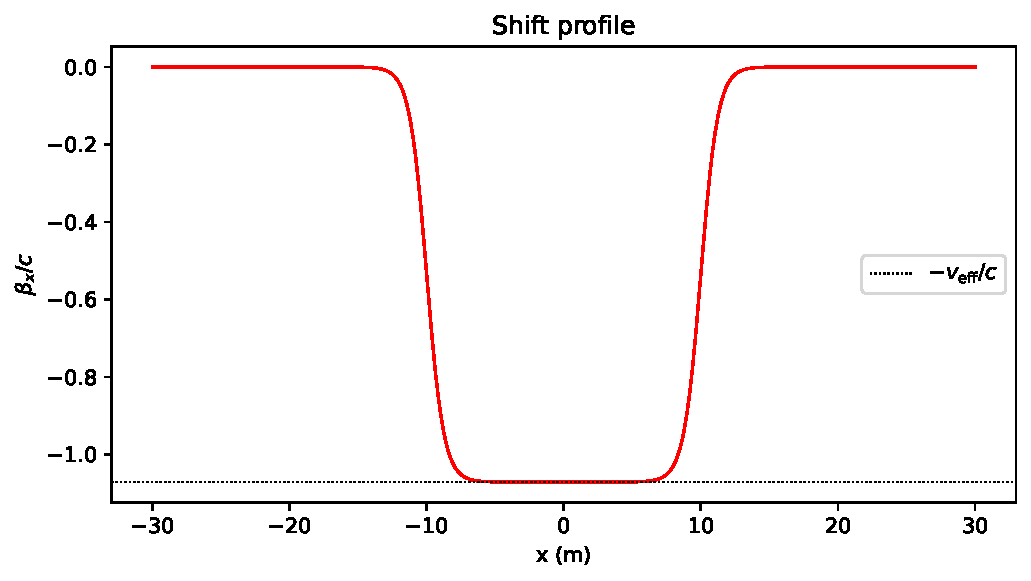
\includegraphics[width=0.86\columnwidth]{figures/shift_profile.pdf}
  \caption{Numerical shift profile generated by the executable extension.
  The interior approaches
  \(\beta_x/c=-\SimOutputWarpVelocity\), while the exterior relaxes to
  zero.}\label{fig:shift-profile}
\end{figure}

\subsection{Fefferman--Graham slice metric}

Use \(\zeta\) for the Fefferman--Graham radial coordinate and
\(x^\mu=(ct,x,y,z)\) for the four-dimensional slice coordinates.  The bulk line element is
\begin{equation}
  ds_5^2
  =
  \frac{L^2}{\zeta^2}
  \left[
    d\zeta^2
    +
    g_{\mu\nu}(\boldsymbol{x},\zeta)
    dx^\mu dx^\nu
  \right].
  \label{eq:five-dimensional-fg-form}
\end{equation}
On the operating slice \(\zeta=\zeta_*\), define the dimensionless shift
\begin{equation}
  b(\boldsymbol{x})
  =
  \frac{\beta_x(\boldsymbol{x})}{c}.
  \label{eq:dimensionless-shift}
\end{equation}
The induced four-dimensional line element is
\begin{equation}
  ds_4^2
  =
  -c^2dt^2
  +
  \left[
    dx+\beta_x(\boldsymbol{x})dt
  \right]^2
  +
  dy^2
  +
  dz^2.
  \label{eq:four-dimensional-shift-line-element}
\end{equation}
In coordinates \(x^\mu=(ct,x,y,z)\), its covariant matrix is
\begin{equation}
  g_{\mu\nu}^{\mathrm L}
  =
  \begin{pmatrix}
    -1+b^2 & b & 0 & 0 \\
    b & 1 & 0 & 0 \\
    0 & 0 & 1 & 0 \\
    0 & 0 & 0 & 1
  \end{pmatrix}.
  \label{eq:lorentzian-shift-matrix}
\end{equation}
Direct evaluation gives
\begin{equation}
  \det g^{\mathrm L}
  =
  \left(-1+b^2\right)-b^2
  =
  -1,
  \label{eq:lorentzian-determinant}
\end{equation}
or \(\det g^{\mathrm L}=-c^2\) when \(t\), rather than \(ct\), is used as the temporal coordinate.  Hence the Lorentzian slice is nonsingular for every finite shift.  The numerical grid audit reports
\begin{equation}
  \min_{\boldsymbol{x}}
  \left|
    \det g^{\mathrm L}(\boldsymbol{x})
  \right|
  =
  \SimOutputMetricDetMin.
  \label{eq:numerical-determinant-audit}
\end{equation}

\subsection{Positive-definite Gram representative}

The Lorentzian metric in Eq.~\eqref{eq:lorentzian-shift-matrix} is necessarily indefinite.  Positive-definiteness applies instead to the Euclidean Gram representative constructed by the holographic projector.  Let \(v_s^a\) be the four orthonormal frame vectors, \(W_s>0\) their interval weights, and \(D=\operatorname{diag}(d_0,d_1,d_2,d_3)\) with \(d_a>0\).  Define
\begin{equation}
  \widetilde g_{ab}
  =
  \sum_{s=0}^{3}
  W_s
  v_{sa}v_{sb}
  +
  D_{ab}.
  \label{eq:weighted-gram-representative}
\end{equation}
For any nonzero real vector \(u\in\mathbb R^4\),
\begin{equation}
  u^a\widetilde g_{ab}u^b
  =
  \sum_{s=0}^{3}
  W_s
  \left(
    u^a v_{sa}
  \right)^2
  +
  \sum_{a=0}^{3}
  d_a
  (u^a)^2.
  \label{eq:gram-quadratic-form}
\end{equation}
Every term is nonnegative, and the second sum is strictly positive for \(u\neq0\).  Therefore
\begin{equation}
  u^a\widetilde g_{ab}u^b
  \geq
  \left(
    \min_a d_a
  \right)
  \|u\|_2^2
  >0,
  \qquad
  \lambda_{\min}(\widetilde g)
  \geq
  \min_a d_a
  >0.
  \label{eq:gram-positive-definite-proof}
\end{equation}

After symmetrization, eigenvalue regularization, and trace normalization, the projected representative is
\begin{equation}
  g_{ab}^{\mathrm G}
  =
  \frac{
    \operatorname{Sym}
    \left(
      \widetilde g_{ab}
      +
      \epsilon_{\mathrm{eig}}\delta_{ab}
    \right)
  }{
    \operatorname{Tr}
    \left[
      \operatorname{Sym}
      \left(
        \widetilde g
        +
        \epsilon_{\mathrm{eig}}\mathbb I_4
      \right)
    \right]
  },
  \qquad
  \epsilon_{\mathrm{eig}}>0.
  \label{eq:trace-normalized-gram-metric}
\end{equation}
Its trace and minimum eigenvalue satisfy
\begin{equation}
  \operatorname{Tr}g^{\mathrm G}
  =
  1,
  \qquad
  \lambda_{\min}(g^{\mathrm G})
  \geq
  \frac{
    \min_a d_a+\epsilon_{\mathrm{eig}}
  }{
    \operatorname{Tr}\widetilde g
    +
    4\epsilon_{\mathrm{eig}}
  }
  >0.
  \label{eq:normalized-gram-positivity}
\end{equation}
The executable audit obtains
\begin{equation}
  \min_{\boldsymbol{x}}
  \lambda_{\min}
  \left(
    g^{\mathrm G}(\boldsymbol{x})
  \right)
  =
  \SimOutputMetricEigenMin.
  \label{eq:numerical-gram-eigenvalue}
\end{equation}
Equations~\eqref{eq:lorentzian-determinant} and~\eqref{eq:normalized-gram-positivity} establish the two required properties without conflating signatures: the physical ADM slice is Lorentzian and nonsingular, whereas the holographic projection representative is symmetric and positive definite.